\documentclass[twocolumn]{article}
\usepackage[utf8]{inputenc}
\usepackage{amsmath}
\usepackage{algorithm}
\usepackage{tikz}
\usepackage{dblfloatfix}
\usepackage[noend]{algpseudocode}
\usetikzlibrary{shapes.arrows}
\usepackage{xcolor}
\makeatletter
\def\BState{\State\hskip-\ALG@thistlm}
\makeatother
\graphicspath{ {./} }
\definecolor{mygray}{gray}{0.7}
\title{CMPUT652-Assignment4}
\author{Yourui Guo }
\date{April 2019}

\begin{document}
\maketitle

\section{Abstract}
In this work, A * with Bidirectional Pathmax (BPMX) was implemented and tested on domains such as 3D voxel-based pathfinding problem and 2D grid-based pathfinding problem. Experiments applied with Differential Heuristics were tested and compared. The result shows that furthest pivot placement performs well in simple map, and optimized pivot placement performs well in complex map. 

\section{Introduction}

\subsection{A* with BPMX}

A* achieves the best performance in terms of number of node expansions when heuristic is both admissible and consistent. However, inconsistent heuristic can cause node re-expansions as many as $O(2^N)$ node expansions [2] where N is the number of distinct expanded nodes. Pathmax is introduced to keep f-values along any path in graph monotonic non-decreasing. The basic idea of pathmax is to propagate heuristic values from parent node to child node if parent node has a larger heuristic value.

BPMX propagates heuristic values from the node with large heuristic to any direction. Nodes along the traversed path are updated with the subtraction of large heuristic and the actual cost along the way. The update process only stops when the node has a larger original heuristic than propagated value. A* was implemented with one-step BPMX where one parent and its children are propagated with the maximum heuristic among them at one time.


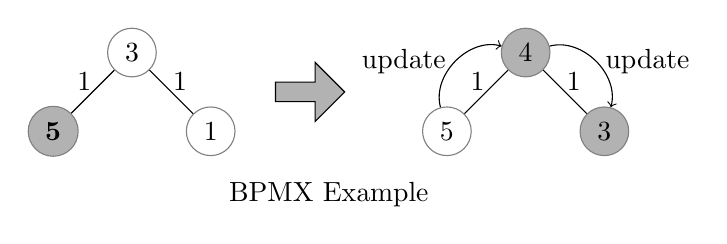
\begin{tikzpicture}
  [state/.style={circle,draw=gray},
   red/.style={fill=mygray},
   update/.style={fill=mygray},
   towards/.style={->},
   arrow/.style = {
    single arrow, draw,
    minimum height=2.5em,
    transform shape,
    fill=mygray,
  },
   bend angle =60,
  ]
  
  \node[state] (n0) at (2,1.5)  {3};
  \node[state, red] (n1) at (1,0.5)  {\textbf{5}};
  \node[state] (n2) at (3,0.5)  {1};

  \node[arrow] (x) at (4.2,1) {};

  \node[state, update] (n3) at (7,1.5)  {4};
  \node[state] (n4) at (6,0.5)  {5};
  \node[state, update] (n5) at (8,0.5)  {3};
  
  \path (n0) edge node[pos=0.7, above]{1} (n1)
        (n0) edge node[pos=0.7, above]{1} (n2)
        (n3) edge node[pos=0.7, above]{1} (n4)
        (n3) edge node[pos=0.7, above]{1} (n5)
        (n4) edge[towards, bend left] node[left]{update} (n3)
        (n3) edge[towards, bend left] node[right]{update} (n5);
  
  \node (a) at(4.5, -0.3) {BPMX Example};
    
\end{tikzpicture}

\begin{algorithm}
\caption{A* with BPMX}\label{euclid}
\begin{algorithmic}[1]
\State $openlist[0] \gets \text{start}$
\While{\textit{openlist} != NULL}
\State $state \gets$ min($openlist$)
\If{$state$ is goal} $return$\EndIf
\While {action \text{in next actions}}
    \State $BestH \gets \text{max}(BestH, state.H-\text{cost})$
\EndWhile
\State $state.H \gets \text{max}(BestH, state.H)$
\State  add \textit{state} to $closedlist$
\While {action \text{in next actions}}
    \State $next \gets$\text{applyAction}(\textit{action})
    \If{$next$ in $closedlist$}
        \If{$next.H < BestH - cost$}
            \State $next.H \gets BestH-cost$
        \EndIf
        \If{$state.G + cost < next.G$}
            \State REOPEN $next$
        \EndIf
    \ElsIf{$next$ in openlist}
         \If{$state.G + cost < next.G$}
            \State UPDATE $next$
        \EndIf
        \If{$next.H < BestH - cost$}
            \State $next.H \gets BestH-cost$
        \EndIf
    \Else
        \State add \textit{next} to $openlist$
    \EndIf
\EndWhile
\EndWhile
\end{algorithmic}
\end{algorithm}

A* wih BPMX performs well with inconsistent heuristic and reduces number of node expansions comparing to A*.  The f-function of inconsistent heuristic is non-monotonic so that A* might re-expand nodes when they can be reached through a path with lower cost. It requires A* to expands nodes and move nodes to closed list, and then re-open nodes and add them to open list again. By applying BPMX, number of node re-expansions drops and the f-function along the traversed paths is monotonically non-decreasing. 




\subsection{Differential Heuristic}

Differential Heuristic selects one pivot as a point that calculates all actual cost from any point in the map to it. Heuristic function is the subtraction of actual costs from any two points to the pivot, which can be presented as h(a, b) = | d(a, s) - d(b, s) | where s is the pivot, and a, b are any point in the map. The cost from pivot to all other states in map is calculated by Dijkstra’s algorithm. Differential Heuristic performs perfect when it gives the true distance heuristic to a pair of points. When the pivot is on the side beyond goal/start state along the optimal path to the start/goal state, the given heuristic is the true distance from start state to goal state. However, Differential Heuristic might perform badly when the pivot is in the middle of the optimal path from start state to goal state. In this case, the heuristic between two points is 0 even their true distance is larger than 0. 

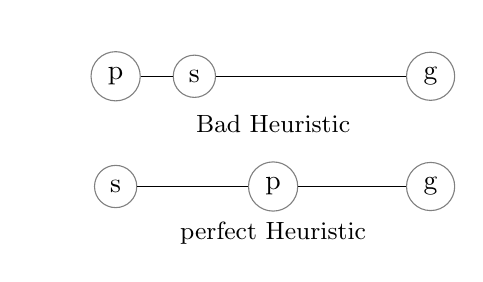
\begin{tikzpicture}
  [state/.style={circle,draw=gray},
   bend angle =60,
  ]
  \node (a) at (0,2.7){};
  \node (a) at (0,0.2){};
  \node[state] (n0) at (2,2.2)  {s};
  \node[state] (n1) at (1,2.2)  {p};
  \node[state] (n2) at (5,2.2)  {g};


  \node[state] (n3) at (1,0.8)  {s};
  \node[state] (n4) at (3,0.8)  {p};
  \node[state] (n5) at (5,0.8)  {g};
  
  \path (n0) edge node[pos=0.7, above]{} (n1)
        (n0) edge node[pos=0.7, above]{} (n2)
        (n3) edge node[pos=0.7, above]{} (n4)
        (n4) edge node[pos=0.7, above]{} (n5);
  
  \node (a) at(3, 1.6) {\small Bad Heuristic};
  \node (a) at(3, 0.2) {\small perfect Heuristic};
    
\end{tikzpicture}


There are three strategies to place the pivot which are random placement, furthest placement and optimized placement. Random placement generates pivots by selecting states randomly from the map. Furthest placement generates a pivot randomly at first, and apply Dijkstra’s algorithm to find the last expanded state in the map. Then, the last expanded state is set as the first pivot to find out the next pivot. The last pivot is generated by adding all generated furthest pivots to the open list at the beginning of Dijkstra’s search and finding out the last expanded state in the map. Optimized placement generates multiple furthest pivots and then measure the gain of each differential heuristic comparing to default heuristic from sample states. Pivots with large heuristic gain will be considered as optimized pivots. In this work, the default heuristic for 3D voxel-based pathfinding problem is voxel heuristic, and the default heuristic for 2D grid-based pathfinding problem is octile heuristic. 


\section{Implementation}

\subsection{3D Voxel-Based Path Finding}

Voxels are volume elements in 3D space, where they are equivalent to pixels in 2D space. The state of voxel can be represented by the tuple of $[x, y, z]$ where $x, y, z$ are coordinates in 3 dimensional space. Start state and goal state are given in benchmark, and coordinates listed in map are filled states.  State is hashed by ranking, and the formula of ranking is: \begin{equation}
    s_{rank} = ((s_x*size_y)+s_y)*size_z.
\end{equation} 

For each state, there are 26 possible actions where the cost of each action can be different. There are three types of actions which are moving along single coordinate, moving two coordinates and moving three coordinates. All possible actions can be represented by the permutations of [$\delta$x, $\delta$y, $\delta$z] where each element has value of -1, 0 and 1,  excluding action being [0, 0, 0]. The cost of moving single coordinate is 1, and the cost of moving two coordinates is $\sqrt{2}$, and the cost of moving three coordinates is $\sqrt{3}$. For last two moving situations, we have to guarantee that no voxel is filled on the path from current node to next adjacent node by moving one single coordinate at a time.

The heuristic function in 3d voxel-based path finding is voxel heuristic. Given two nodes and their distances of $\delta$x, $\delta$y and $\delta$z, the voxel heuristic is
\begin{equation}
H_{voxel} = (\sqrt{3}-\sqrt{2})d_{min} + (\sqrt{2}-1)d_{mid} + d_{max}
\end{equation}

where
\begin{gather*}
    d_{min} = min(\delta x, \delta y, \delta z), \\
    d_{max} = max(\delta x, \delta y, \delta z), \\
    d_{mid} = \{\delta x, \delta y, \delta z\} \setminus \{d_{max}, d_{min}\}.
\end{gather*}

\subsection{2D Grid-Based Path Finding}

Grid-based environment is composed of grids, where each grid has 8 adjacent states. The state of grid can be represented by coordinate [x, y], and it is hashed by ranking. The formula of ranking the state is \begin{equation}
    s_{rank} = s_x * size_y + s_y
\end{equation} . Each state has 8 actions,  and all possible actions can be represented by the permutations of [δx, δy] where each element has value of -1, 0 and 1, excluding action being [0, 0]. Action is not allowed when the next state is filled or it cuts corners through obstacle.  Start state and goal state are given in benchmark, and coordinates listed in map are filled states.  

The default heuristic function in 2D grid-based path finding is octile heuristic. Given two nodes and their distances of x and y, the heuristic is 
\begin{equation}
H_{octile} = (\sqrt{2}-1)d_{min} + d_{max}
\end{equation}

where
\begin{gather*}
    d_{min} = min(\delta x, \delta y), \\
    d_{max} = max(\delta x, \delta y), \\
\end{gather*}

\subsection{Heuristic Lookup}


In this work, experiments are tested with three different strategies of heuristic lookup. There are 10 pivots generated when building the database of Differential Heuristic. Single consistent lookup is to select one heuristic from the database where the pivot that provides the heuristic is consistent during search. Single inconsistent lookup is to select one heuristic from database randomly, in which heuristics of different states are calculated from different pivots. The last strategy is multiple lookup, which is to select the maximum value among 10 heuristics. Heuristic from different lookup strategies will be compared with voxel/octile heuristic and choose the maximum between them.

Single consistent lookup and multiple lookup provide consistent heuristic, while single inconsistent random lookup provides inconsistent heuristic. So, in this work, only single inconsistent lookup strategy was tested with A* with BPMX.


\subsection{Data Structure}
Efficient data structure was applied to implement A* algorithm and NBS algorithm. Priority queue is aimed at reducing running time for sorting open-list. Priority queue is maintained by binary heap, in which functionalities of push, pop and peak are provided. In NBS, there are 4 priority queues which are forward and backward waiting lists along with forward and backward ready lists. Forward/Backward open-list is the set union of forward/backward waiting list and ready list. The running time for each priority queue reduces from O(N) to O(log(N)).


\begin{algorithm}
\caption{Priority Queue}\label{euclid}
\begin{algorithmic}[1]
\Procedure{Push}{}
\State $ \textit{heap\_len} \gets \text{length of heap}$
\State $ heap[\textit{heap\_len-1}] \gets \text{value} $
\State $ \textit{i} \gets \textit{heap\_len} $
\While{$\textit{(i-1)}/2 >= 0$}

\If{$\textit{heap[i]} < \textit{heap[(i-1)/2]}$} 
\State $\text{swap(} \textit{i}, \textit{(i-1)/2})$
\EndIf
\If{$\textit{heap[i]} == \textit{heap[(i-1)/2]}$} 
    \If{$gcost(\textit{i}) > gcost(\textit{(i-1)/2})$}
        \State $\text{swap(} \textit{i}, \textit{(i-1)/2})$
    \EndIf
\EndIf
\State $ \textit{i} \gets \textit{i/2} $
\EndWhile
\EndProcedure
\end{algorithmic}
\end{algorithm}


\begin{algorithm}
\caption{Priority Queue}\label{euclid}
\begin{algorithmic}[1]
\Procedure{Pop}{}

\State $ \textit{heap\_len} \gets \text{length of heap}$
\State $ \text{value} \gets  heap[0] $
\State $ heap[0] \gets  heap[\textit{heap\_len-1}]  $
\State $ \text{delete} (heap[\textit{heap\_len-1}]) $
\While{$\textit{i*2+1} < 0$}
\State $ \textit{index} \gets  \text{min\_child}(i*2+1, i*2+2) $
\If{$heap[i] > heap[index]$} 
\State $\text{swap(} \textit{i}, \textit{index})$
\EndIf
\EndWhile
\EndProcedure
\end{algorithmic}
\end{algorithm}


\section{Experiment}
\begin{table*}[!bhtpH]
\caption{Results for voxel-based pathfinding problem}
\begin{tabular}{|l|l|l|l|l|l|l|}
\hline
Heuristic & Lookup & Solved & Generated & Expanded & Updated & Time elapsed \\ \hline
Optimized & Multiple & 1000/1000 & 792.229 & 344.221 & 395.023 & 0.162 \\ \hline
Optimized & Consistent & 1000/1000 & 1200.145 & 638.487 & 647.643 & 0.359 \\ \hline
Optimized & Inconsistent & 1000/1000 & 1152.912 & 672.557 & 775.061 & 0.474 \\ \hline
Furthest & Multiple & 1000/1000 & 586.46 & 200.3 & 271.76 & 0.204 \\ \hline
Random & Multiple & 1000/1000 & 856.011 & 430.215 & 393.169 & 0.405 \\ \hline
\end{tabular}
\end{table*}

\begin{table*}[!bhtpH]
\caption{Results for grid-based pathfinding problem}
\begin{tabular}{|l|l|l|l|l|l|l|}
\hline
Heuristic & Lookup & Solved & Generated & Expanded & Updated & Time elapsed \\ \hline
Optimized & Multiple & 1572/1572 & 4418.159 & 3681.308 & 1585.931 & 0.408 \\ \hline
Optimized & Consistent & 1572/1572 & 6048.689 & 5423.435 & 2682.580 & 0.564 \\ \hline
Optimized & Inconsistent & 1572/1572 & 9189.643 & 11409.249 & 5490.280 & 1.549 \\ \hline
Furthest & Multiple & 1572/1572 & 4603.279 & 3898.568 & 1758.722 & 0.443 \\ \hline
Random & Multiple & 1572/1572 & 6439.668 & 5756.216 & 2741.767 & 0.599 \\ \hline
\end{tabular}
\end{table*}

Experiments ran on a machine where processor is intel Core i7-8550U CPU @ 1.80GHz 8. The benchmark used for voxel-based pathfinding problem is the simple map where the map dimension is 105x132x105 and the number of total states is 1,454,787. The benchmark used for grid-based pathfinding problem is map brc101d from Dragon Age where the map dimension is 639x384, the number of total states is 29,882 and the maximum path length is 626.57. 

\begin{figure}[h]
\caption{voxel simple map}
\centering
\includegraphics[scale=0.25]{voxel.png}
\end{figure}

\begin{figure}[h]
\caption{grid map}
\centering
\includegraphics[scale=0.25]{brc101d.png}
\end{figure}

Table 1 shows the result from voxel-based pathfinding instances, and we can find that the experiment with furthest pivot placement and multiple heuristic lookup has the minimum number of node expansions comparing to experiment with optimized pivot placement and multiple heuristic lookup along with random pivot placement and multiple heuristic lookup. The optimized placement didn't perform the best might because the tested map is too easy to solve, so that furthest pivot placement was able to provide good heuristic. By applying the same strategy of optimized pivot placement, multiple heuristic lookup hash the minimum number of node expansions and inconsistent heuristic has the maximum number of node expansions. Multiple heuristic lookup outperforms other two strategies is because inconsistent heuristic requires node re-expansions, and single consistent heuristic is not strong enough.


From the table 2 above we can find that the experiment with optimized pivot placement and multiple heuristic lookup has the minimum number of node expansions comparing to experiment with furthest pivot placement and multiple heuristic lookup along with random pivot placement and multiple heuristic lookup. By applying the same strategy of optimized pivot placement, multiple heuristic lookup has the minimum number of node expansions and inconsistent heuristic has the maximum number of node expansions. 

\section{Conclusion}

In this work, we have tested multiple differential heuristic on A* with BPMX, and found out that random pivot placement performs badly on generating heuristic. Furthest pivot placement performs well in simple map, and optimized pivot placement performs well in complex map. BPMX is able to help reducing number of node re-expansions when the heuristic is inconsistent. Due to the hardware limit, this experiment was only tested with simple maps. It should be improved by testing on multiple complex maps to get a more promising result and conclusion.

\section{Reference}

[1] Sturtevant, N. R. and Felner, A. and Barer, M. and Schaeffer, J. and Burch, N..
\textit{Memory-based heuristics for explicit state spaces}
International Joint Conference on Artificial Intelligence (IJCAI), 609--614, 2009.
\newline

[2] Felner, A. and Zahavi, U. and Holte, R. and Schaeffer, J. and Sturtevant, N. and Zhang, Z.
\textit{Inconsistent heuristics in theory and practice}
Artificial Intelligence (AIJ), 2011.
\newline

\end{document}
